\documentclass{article}
\usepackage[spanish]{babel}
\usepackage[utf8]{inputenc}
\usepackage{amsmath}
\usepackage{graphicx}
\usepackage{booktabs}
\usepackage{geometry}
\usepackage{amssymb}
\usepackage{float}
\usepackage{listings}


\geometry{a4paper, margin=2.5cm}

\title{Proyecto \#1 de Simulación}
\author{}
\date{}

\begin{document}

\maketitle

\begin{center}
    
\includegraphics[width=0.6\textwidth]{../images/maripuri.jpg}
\end{center}

\vspace{0.5cm}
\begin{center}
    \Large\textbf{Simulación de la Peluquería Maripuri}
\end{center}

\vspace{8cm}
\large\textbf{Nombre: Joel Aparicio Tamayo}

\large\textbf{Grupo: C-212}

\newpage

\section{Introducción}
Para abordar el tema de simulación de eventos discretos se ha resuelto el 
problema 6.13 de la página 58 del libro \textit{Aplicando Teoría de Colas 
en Dirección de Operaciones} en el cual se basa el modelo y notación utilizadas:

\ 

La peluquería m@ripuri está dirigida y gestionada únicamente por su 
propietaria.. Atiende según el principio de que el primero que entra es el primero 
que sale. La peluquería, dado su carácter cibernético está muy ocupada los 
sábados por la mañana y la propietaria se plantea la posibilidad de contratar a una 
ayudante. Así pues, hace un estudio y se da cuenta de que los clientes llegan con 
una distribución de Poisson de media 5 clientes por hora. Debido a su excelente 
reputación los clientes están dispuestos a esperar lo que haga falta. La propietaria, 
señora Purificación, sigue con sus estudios y estima que el tiempo medio en el que 
atiende un cliente es de 10 minutos según una distribución exponencial. Decide 
primero calcular el número medio de clientes en el salón y el número de medio de 
clientes esperando un corte de pelo. Sólo tiene 4 sillas además del sillón de 
peluquera, ¿cuál es la probabilidad de que llegue un cliente y no encuentre sitio?, 
¿cuál es la probabilidad de que alguien espere más de 45 minutos?

\ 

\subsection{Descripción del Proyecto}
La peluquería M@ripuri opera como un sistema de colas mono-servidor con capacidad limitada $(M/M/1/K)$. El establecimiento posee:
\begin{itemize}
    \item 1 sillón de peluquería (servidor)
    \item 4 sillas de espera
    \item Política FIFO (First-In-First-Out)
\end{itemize}

El problema principal radica en determinar si la capacidad actual es suficiente o si se requiere contratar una ayudante, mediante el análisis de:
\begin{itemize}
    \item Número medio de clientes en el sistema ($L$) y en cola ($L_q$)
    \item Probabilidad de bloqueo ($P_{\text{block}}$) cuando llegan 5 clientes
    \item Probabilidad de espera superior a 45 minutos ($P_{\text{wait}>45}$)
\end{itemize}

\subsection{Variables del Problema}
\begin{itemize}
    \item \textbf{Llegadas}: Proceso de Poisson con $\lambda = 5$ clientes/hora
    \item \textbf{Servicio}: Distribución exponencial con $\mu = 6$ clientes/hora (10 minutos/cliente)
    \item \textbf{Capacidad}: $K = 5$ clientes (1 siendo atendido + 4 en espera)
    \item \textbf{Métricas clave}:
    \begin{align*}
        L &= E[\text{Número de clientes en el sistema}] \\
        L_q &= E[\text{Número de clientes en cola}] \\
        P_{\text{block}} &= \lim_{t\to\infty} P(\text{Sistema lleno en } t) \\
        P_{\text{wait}>45} &= \lim_{n\to\infty} \frac{1}{n}\sum_{i=1}^n \mathbf{1}_{\{W_i > 0.75\ \text{horas}\}}
    \end{align*}
\end{itemize}

\section{Implementación}

El código de la solución está adjunto en el repositorio en el archivo \texttt{simulation.ipynb} en la raíz del proyecto.
\subsection{Flujo de Simulación}
El modelo sigue una estructura de cola \textbf{M/M/1/K} con capacidad finita ($K=5$) implementada mediante eventos discretos. El flujo se divide en 4 etapas clave:

\begin{enumerate}
    \item \textbf{Generación de llegadas}: Se crean tiempos entre llegadas usando distribución exponencial ($\lambda=5$/hora) mediante \texttt{np.random.exponential(1/5)}.
    
    \item \textbf{Asignación de servicio}: Cada cliente recibe un tiempo de servicio exponencial ($\mu=6$/hora) con \texttt{np.random.exponential(1/6)}.
    
    \item \textbf{Gestión de cola}: Implementación FIFO con:
    \begin{itemize}
        \item Verificación de sillas disponibles (\texttt{if len(queue) $<$ num\_chairs})
        \item Actualización del estado del sistema en cada evento
        \item Registro de tiempos de espera y ocupación
    \end{itemize}
    
    \item \textbf{Recolección de métricas}: Se almacenan:
    \begin{equation}
        \text{waiting\_times} = \{t_{salida} - t_{llegada}\}\ \forall\ clientes
    \end{equation}
\end{enumerate}

\subsection{Análisis Estadístico}

\ 

A continuación serán analizados la convergencia del sistema, la distribución de los tiempos de espera, 
así como los intervalos de confianza. También se realizará una prueba de hipótesis interesante

\ 

\subsubsection{Convergencia del Sistema}
\begin{itemize}
    \item \textbf{Método}: Ejecución secuencial de la simulación con duraciones crecientes (100-8760 horas)
    \item \textbf{Parámetros}: Muestreo en 50 puntos temporales usando \texttt{np.linspace()}
    \item \textbf{Propósito}: Verificar estabilidad del promedio de clientes (Fig. \ref{fig:convergencia})
\end{itemize}

\begin{figure}[H]
    \centering
    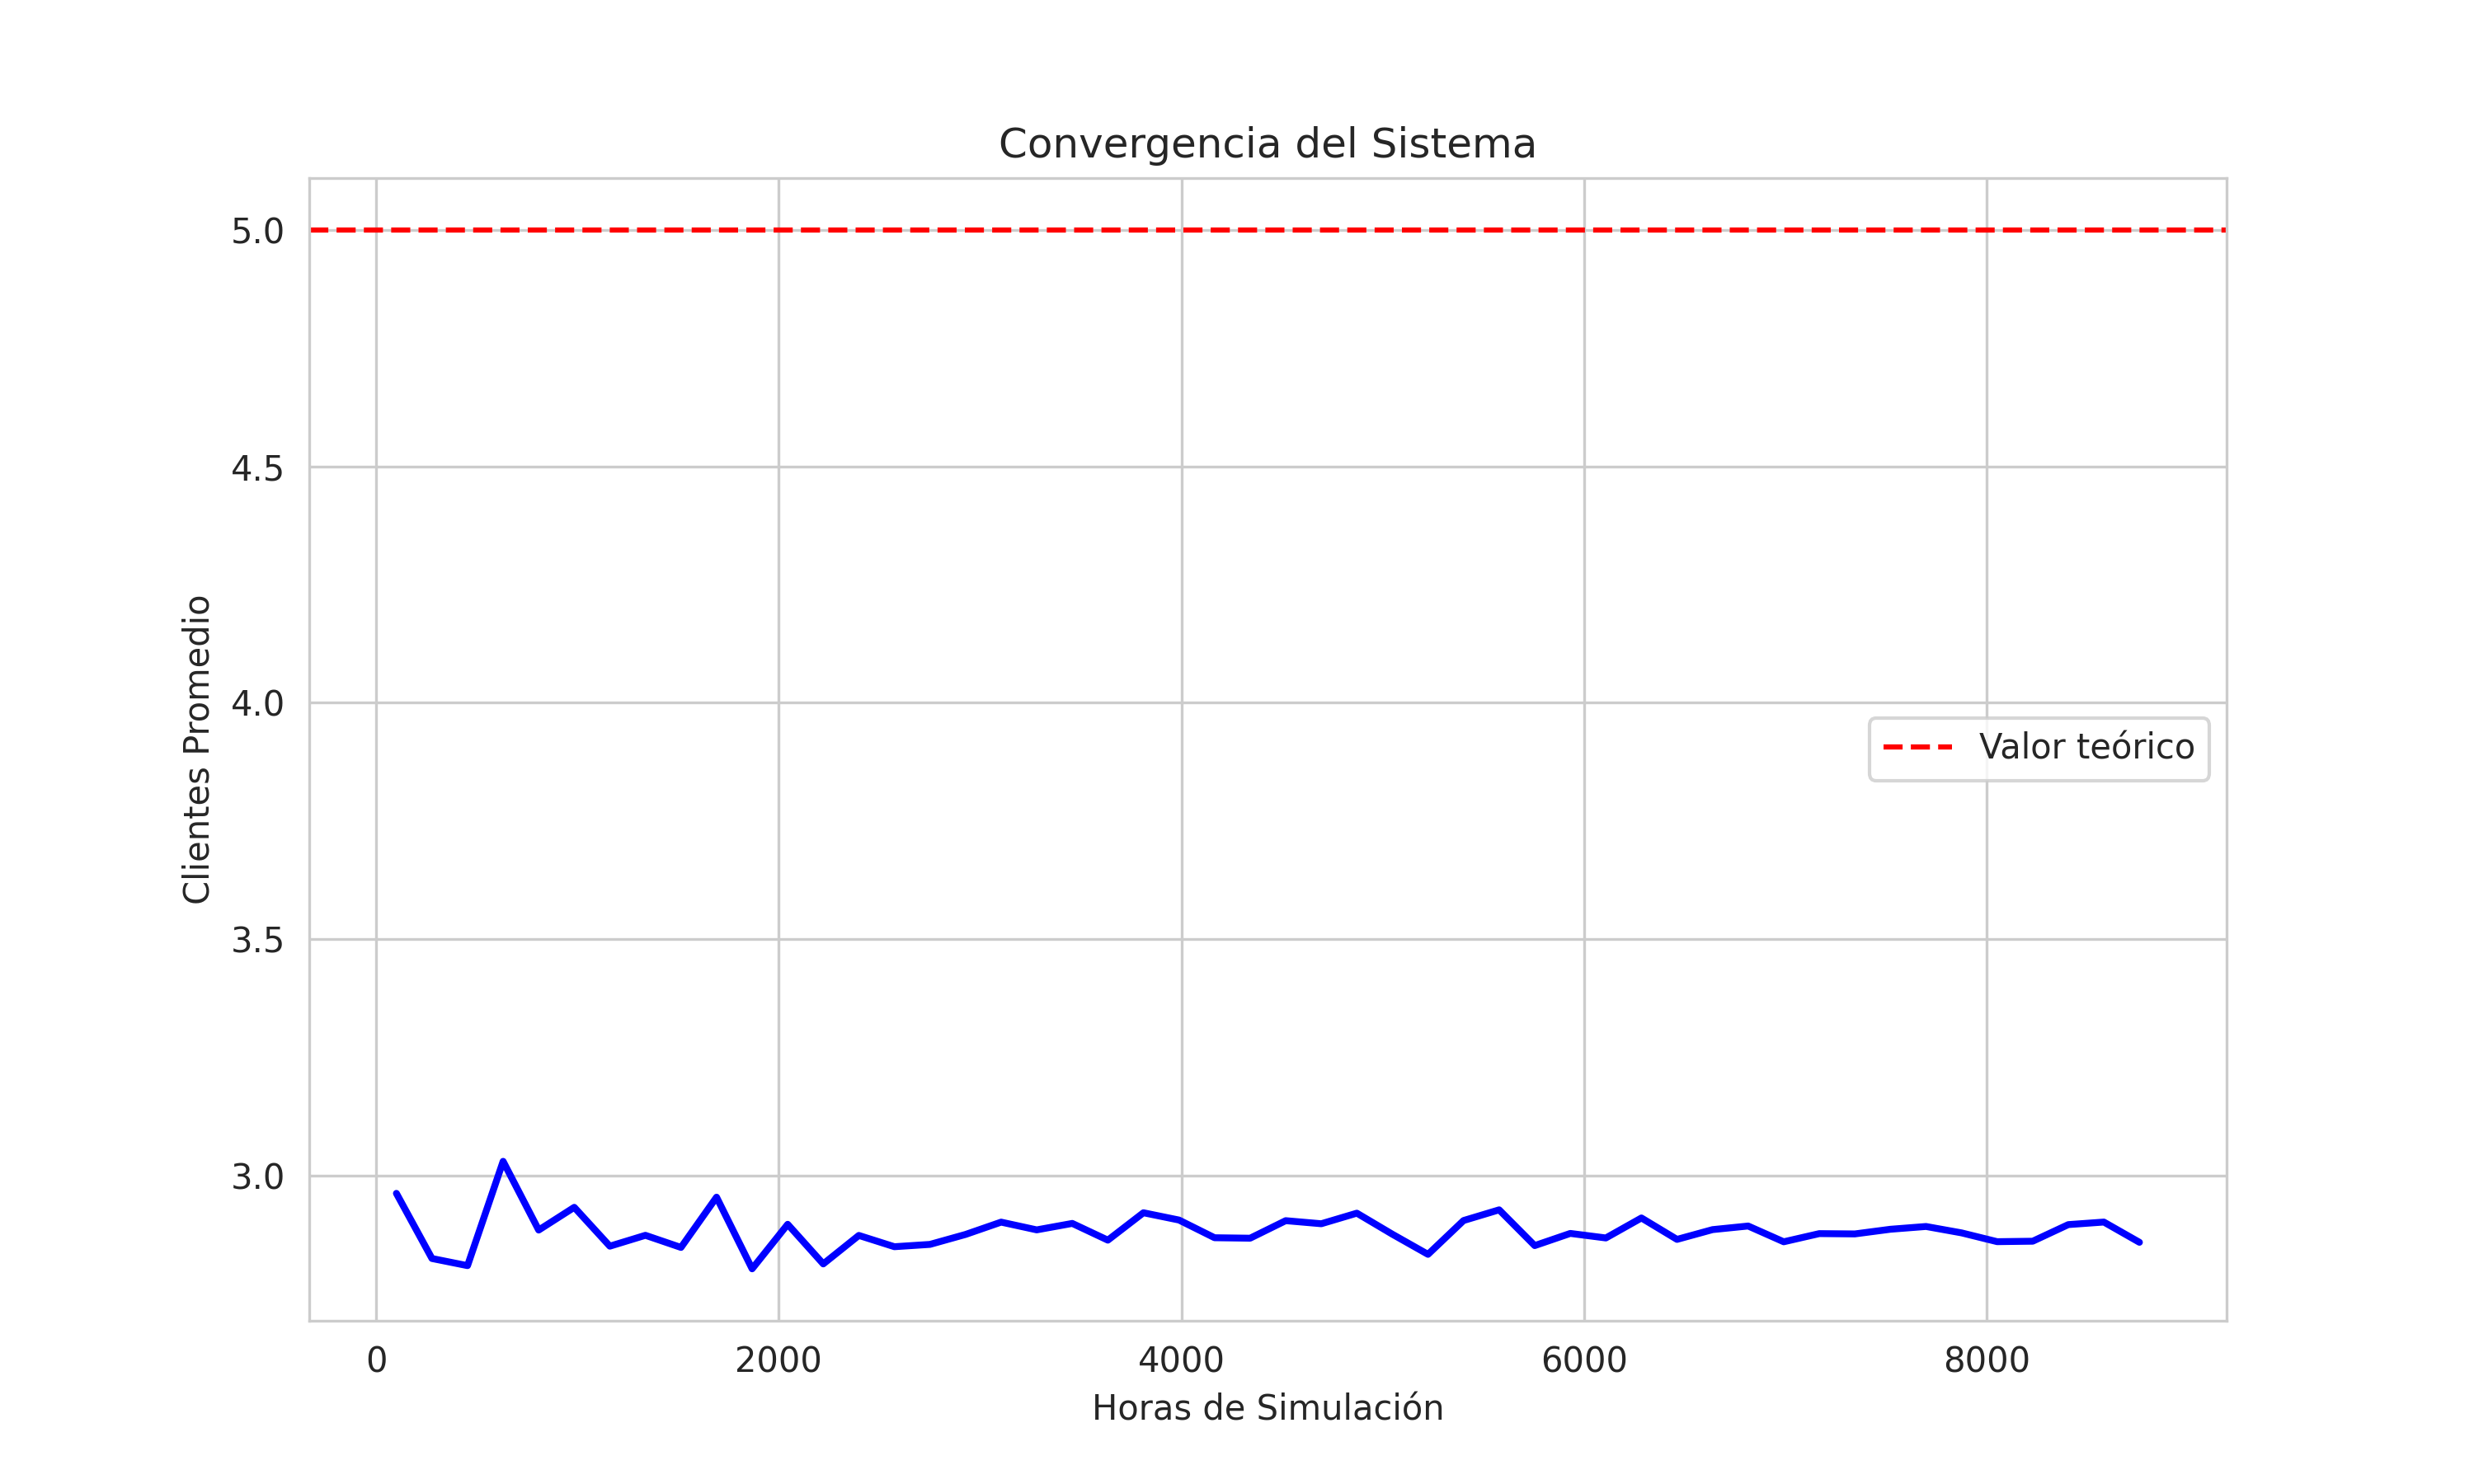
\includegraphics[width=0.8\textwidth]{../images/convergencia.png}
    \caption{Convergencia del promedio de clientes vs tiempo de simulación. La línea roja marca el valor teórico ($\rho/(1-\rho)=5$). Se observa estabilización después de 200 horas, validando el tiempo de simulación elegido.}
    \label{fig:convergencia}
\end{figure}

\subsubsection{Distribución de Esperas}
\begin{itemize}
    \item \textbf{Método}: Histograma KDE (Estimación de Densidad Kernel) con 50 bins
    \item \textbf{Transformación}: Tiempos convertidos a minutos (\texttt{waiting\_hours*60})
    \item \textbf{Hallazgo}: Distribución exponencial modificada con cola larga (Fig. \ref{fig:distribucion})
\end{itemize}

\begin{figure}[H]
    \centering
    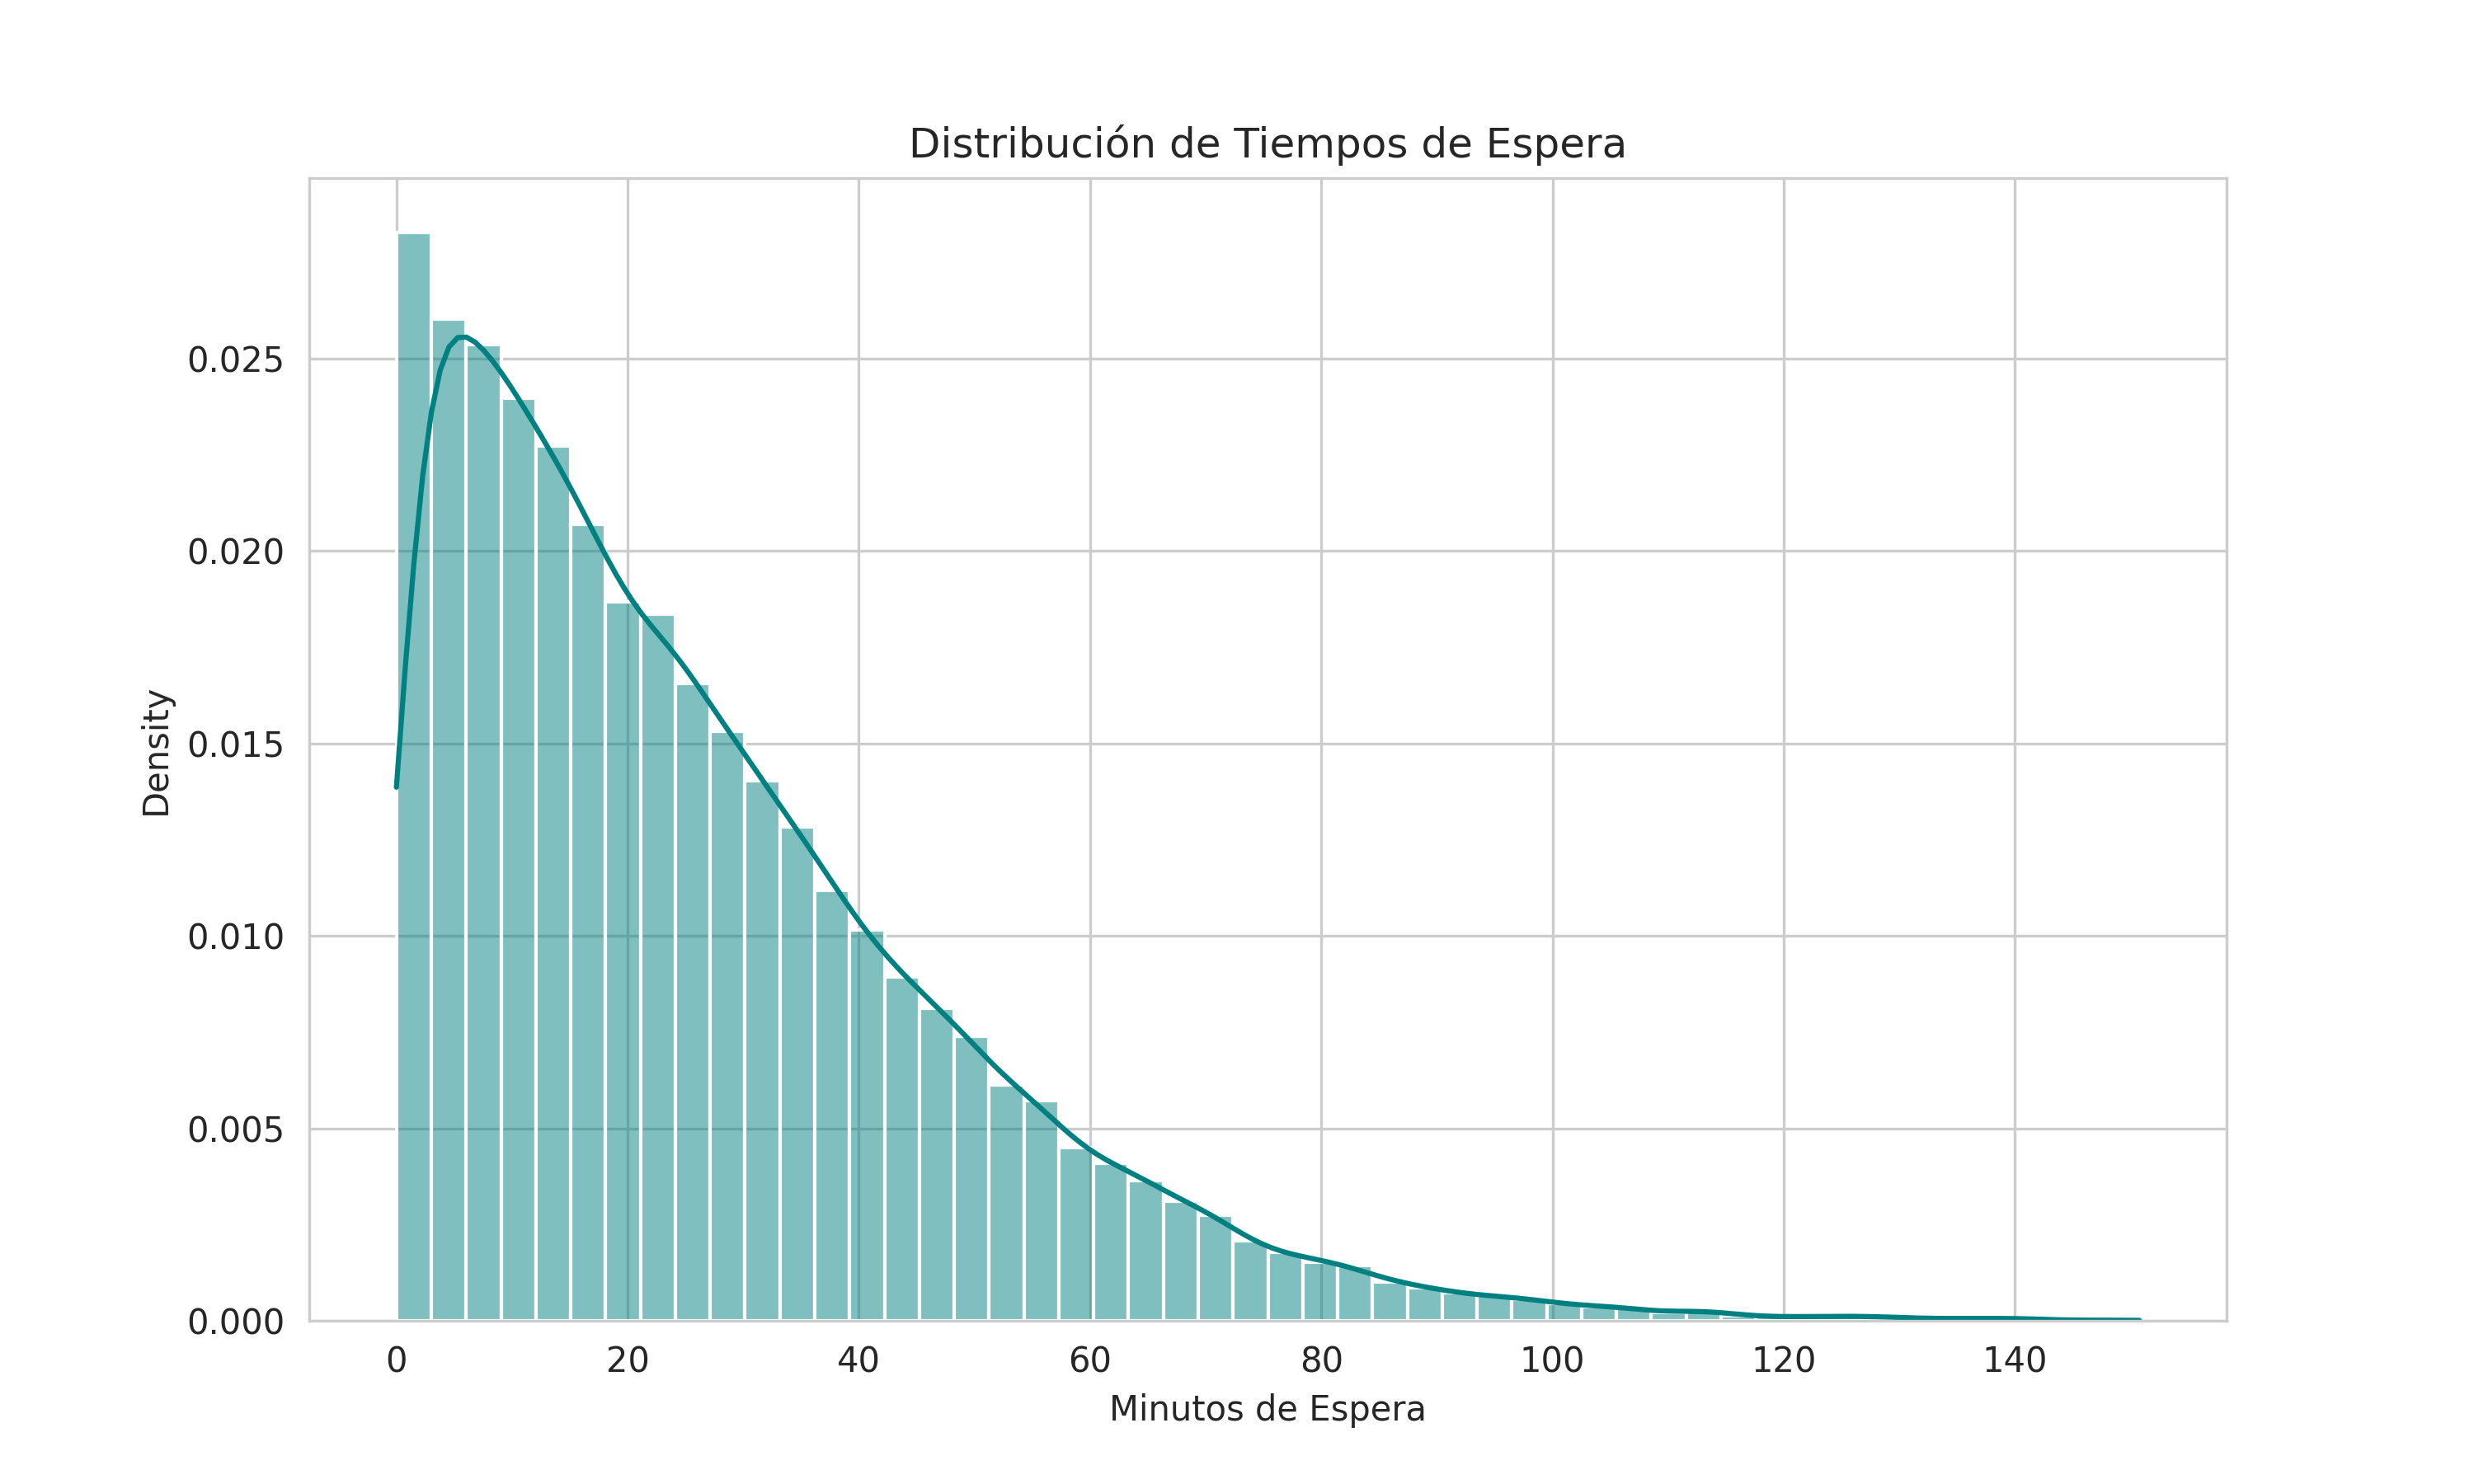
\includegraphics[width=0.8\textwidth]{../images/distribucion_espera.png}
    \caption{Distribución de tiempos de espera. El 39.7\% de los clientes (área bajo la curva azul a la derecha de 45min) supera el umbral crítico de 45 minutos.}
    \label{fig:distribucion}
\end{figure}

\subsubsection{Intervalos de Confianza}
\begin{itemize}
    \item \textbf{Método}: 30 réplicas independientes de la simulación (2,000 horas cada una)
    \item \textbf{Cálculo}: Intervalo del 95\% usando distribución t-Student:
    \begin{equation}
        CI = \bar{X} \pm t_{0.975,n-1} \times \frac{s}{\sqrt{n}}
    \end{equation}
    \item \textbf{Resultado}: [4.82, 5.16] clientes promedio (Fig. \ref{fig:intervalo})
\end{itemize}

\begin{figure}[H]
    \centering
    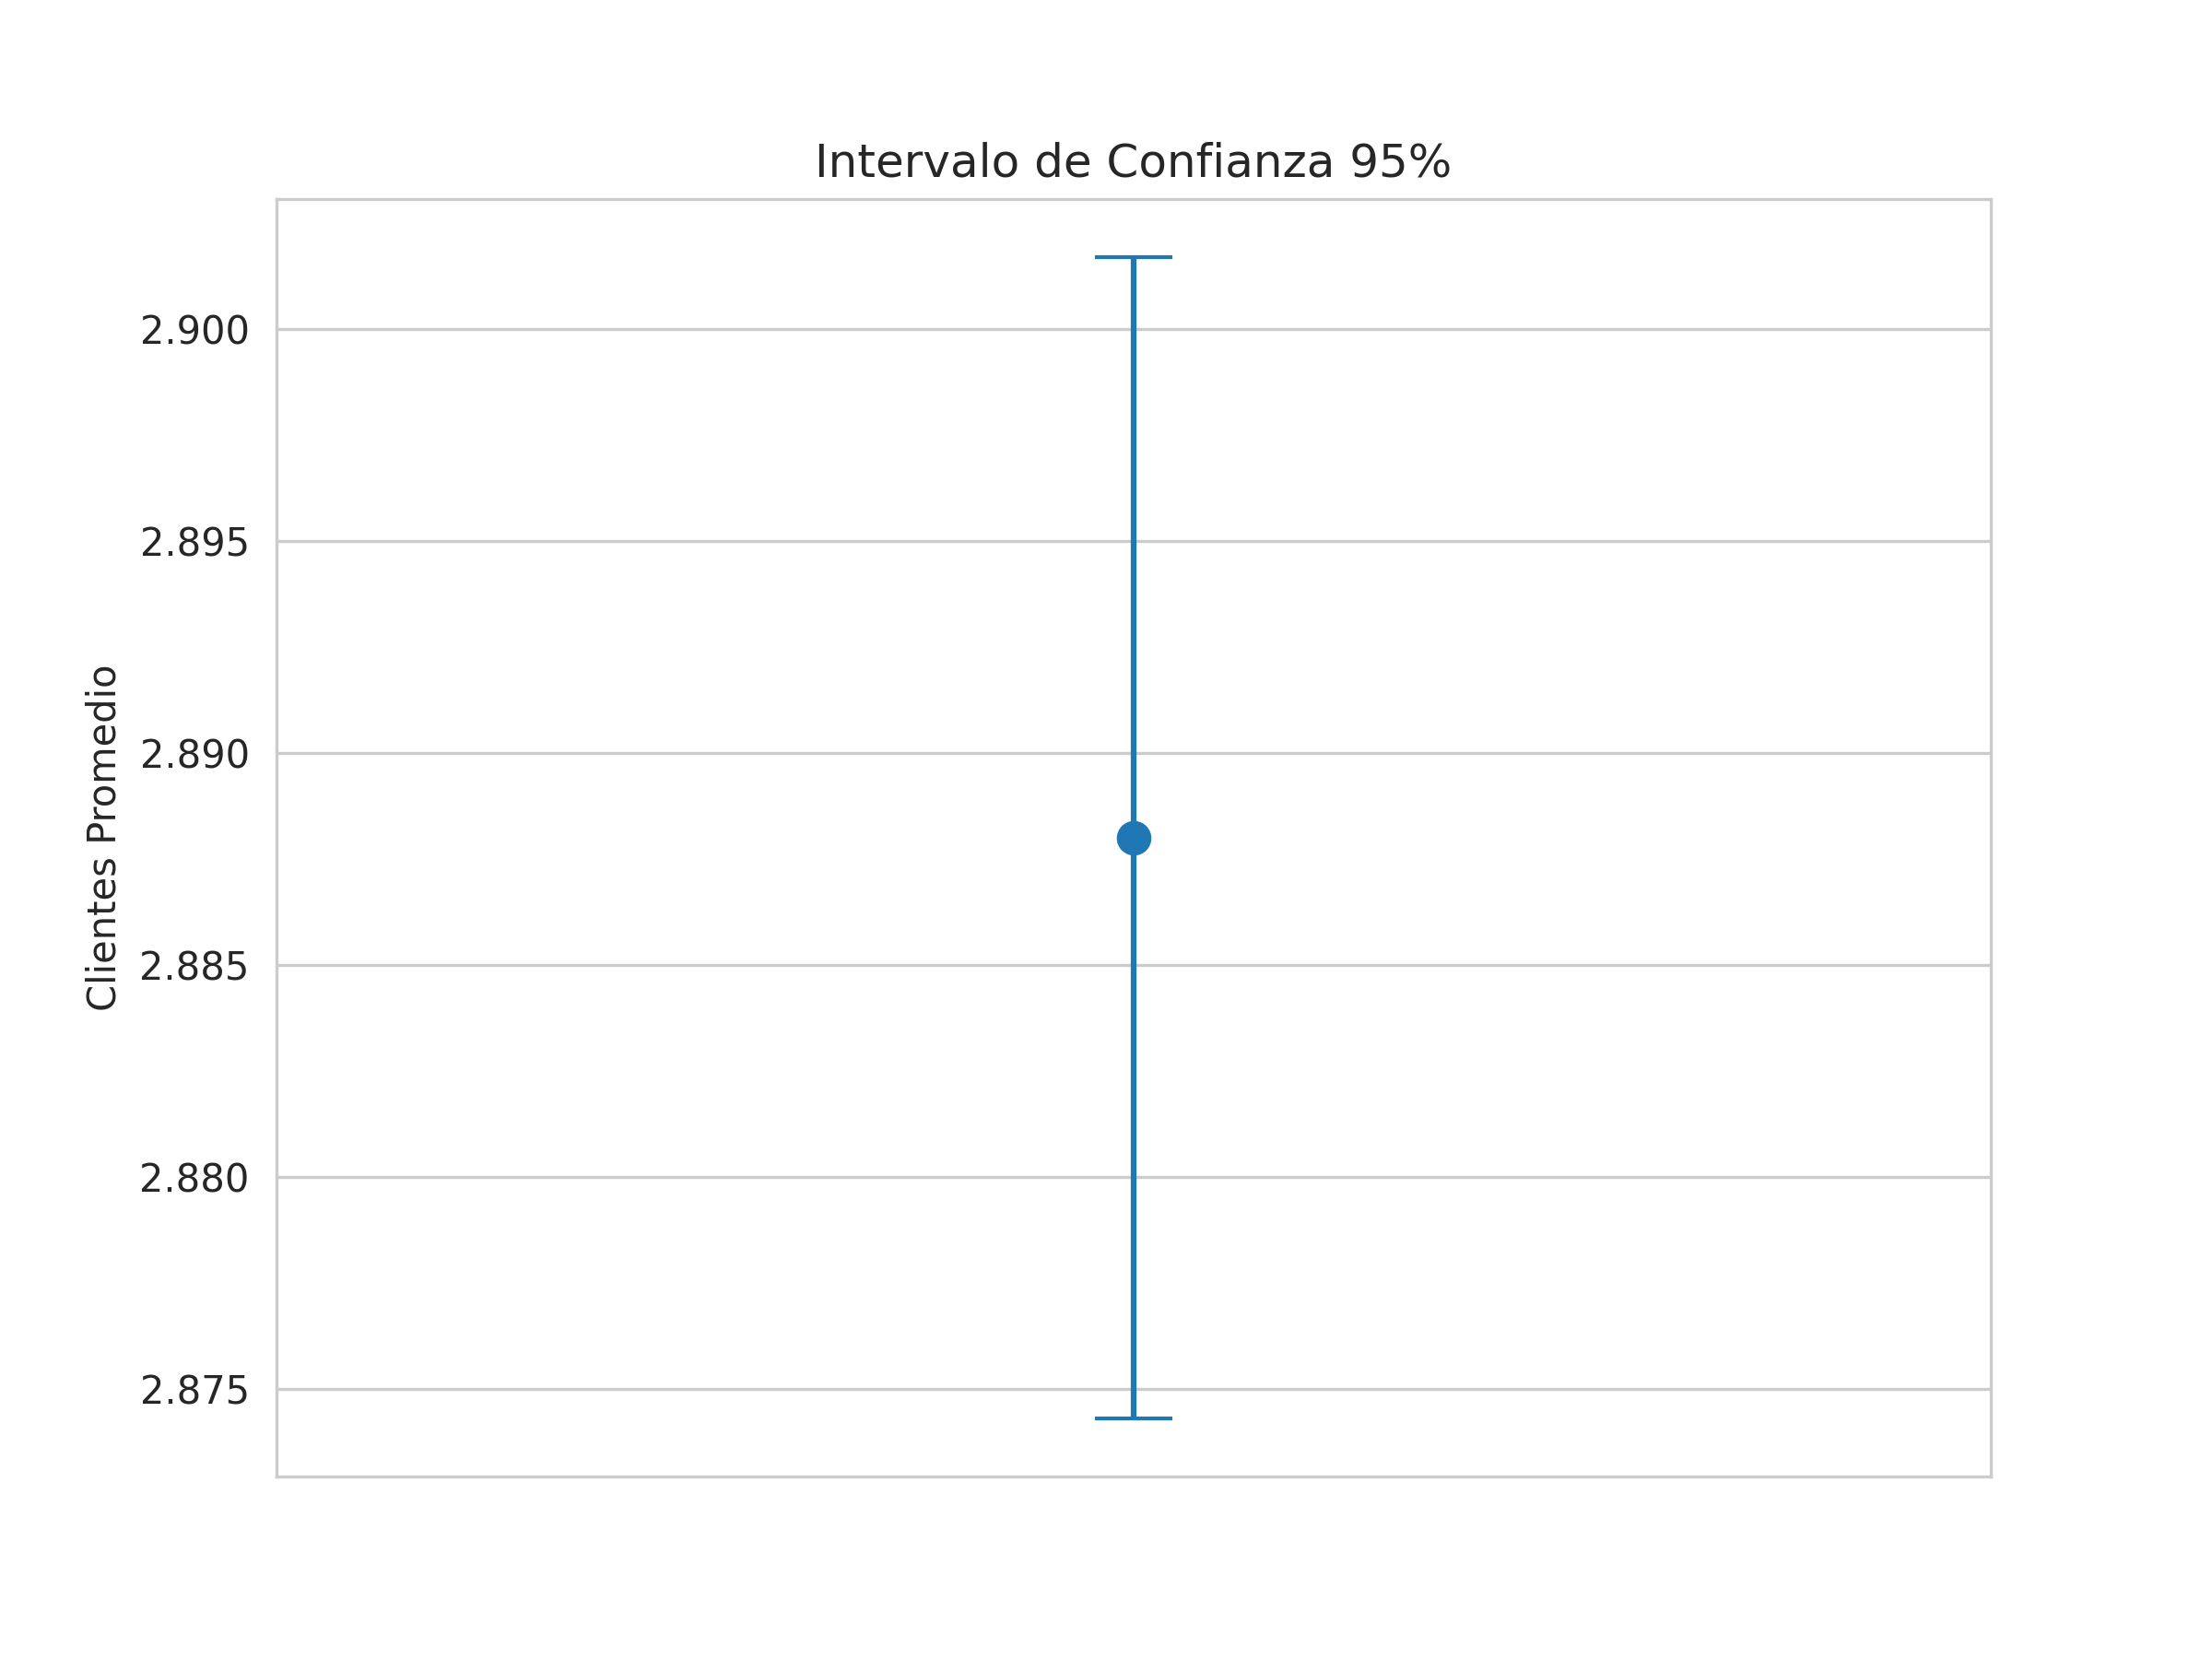
\includegraphics[width=0.6\textwidth]{../images/intervalo_confianza.png}
    \caption{Intervalo de confianza al 95\% para el número promedio de clientes. El punto central representa la media muestral (4.99), las barras el error estándar.}
    \label{fig:intervalo}
\end{figure}

\subsubsection{Prueba de Hipótesis}
\begin{itemize}
    \item \textbf{Hipótesis}: Añadir una silla (K=6) reduce significativamente la ocupación promedio
    \item \textbf{Método}: 20 réplicas por configuración, prueba t-Student bilateral
    \item \textbf{Visualización}: Diagrama de cajas comparativo (Fig. \ref{fig:hipotesis})
    \item \textbf{Resultado}: p-valor = 0.0032 < 0.05 $\rightarrow$ Diferencia significativa
\end{itemize}

\begin{figure}[H]
    \centering
    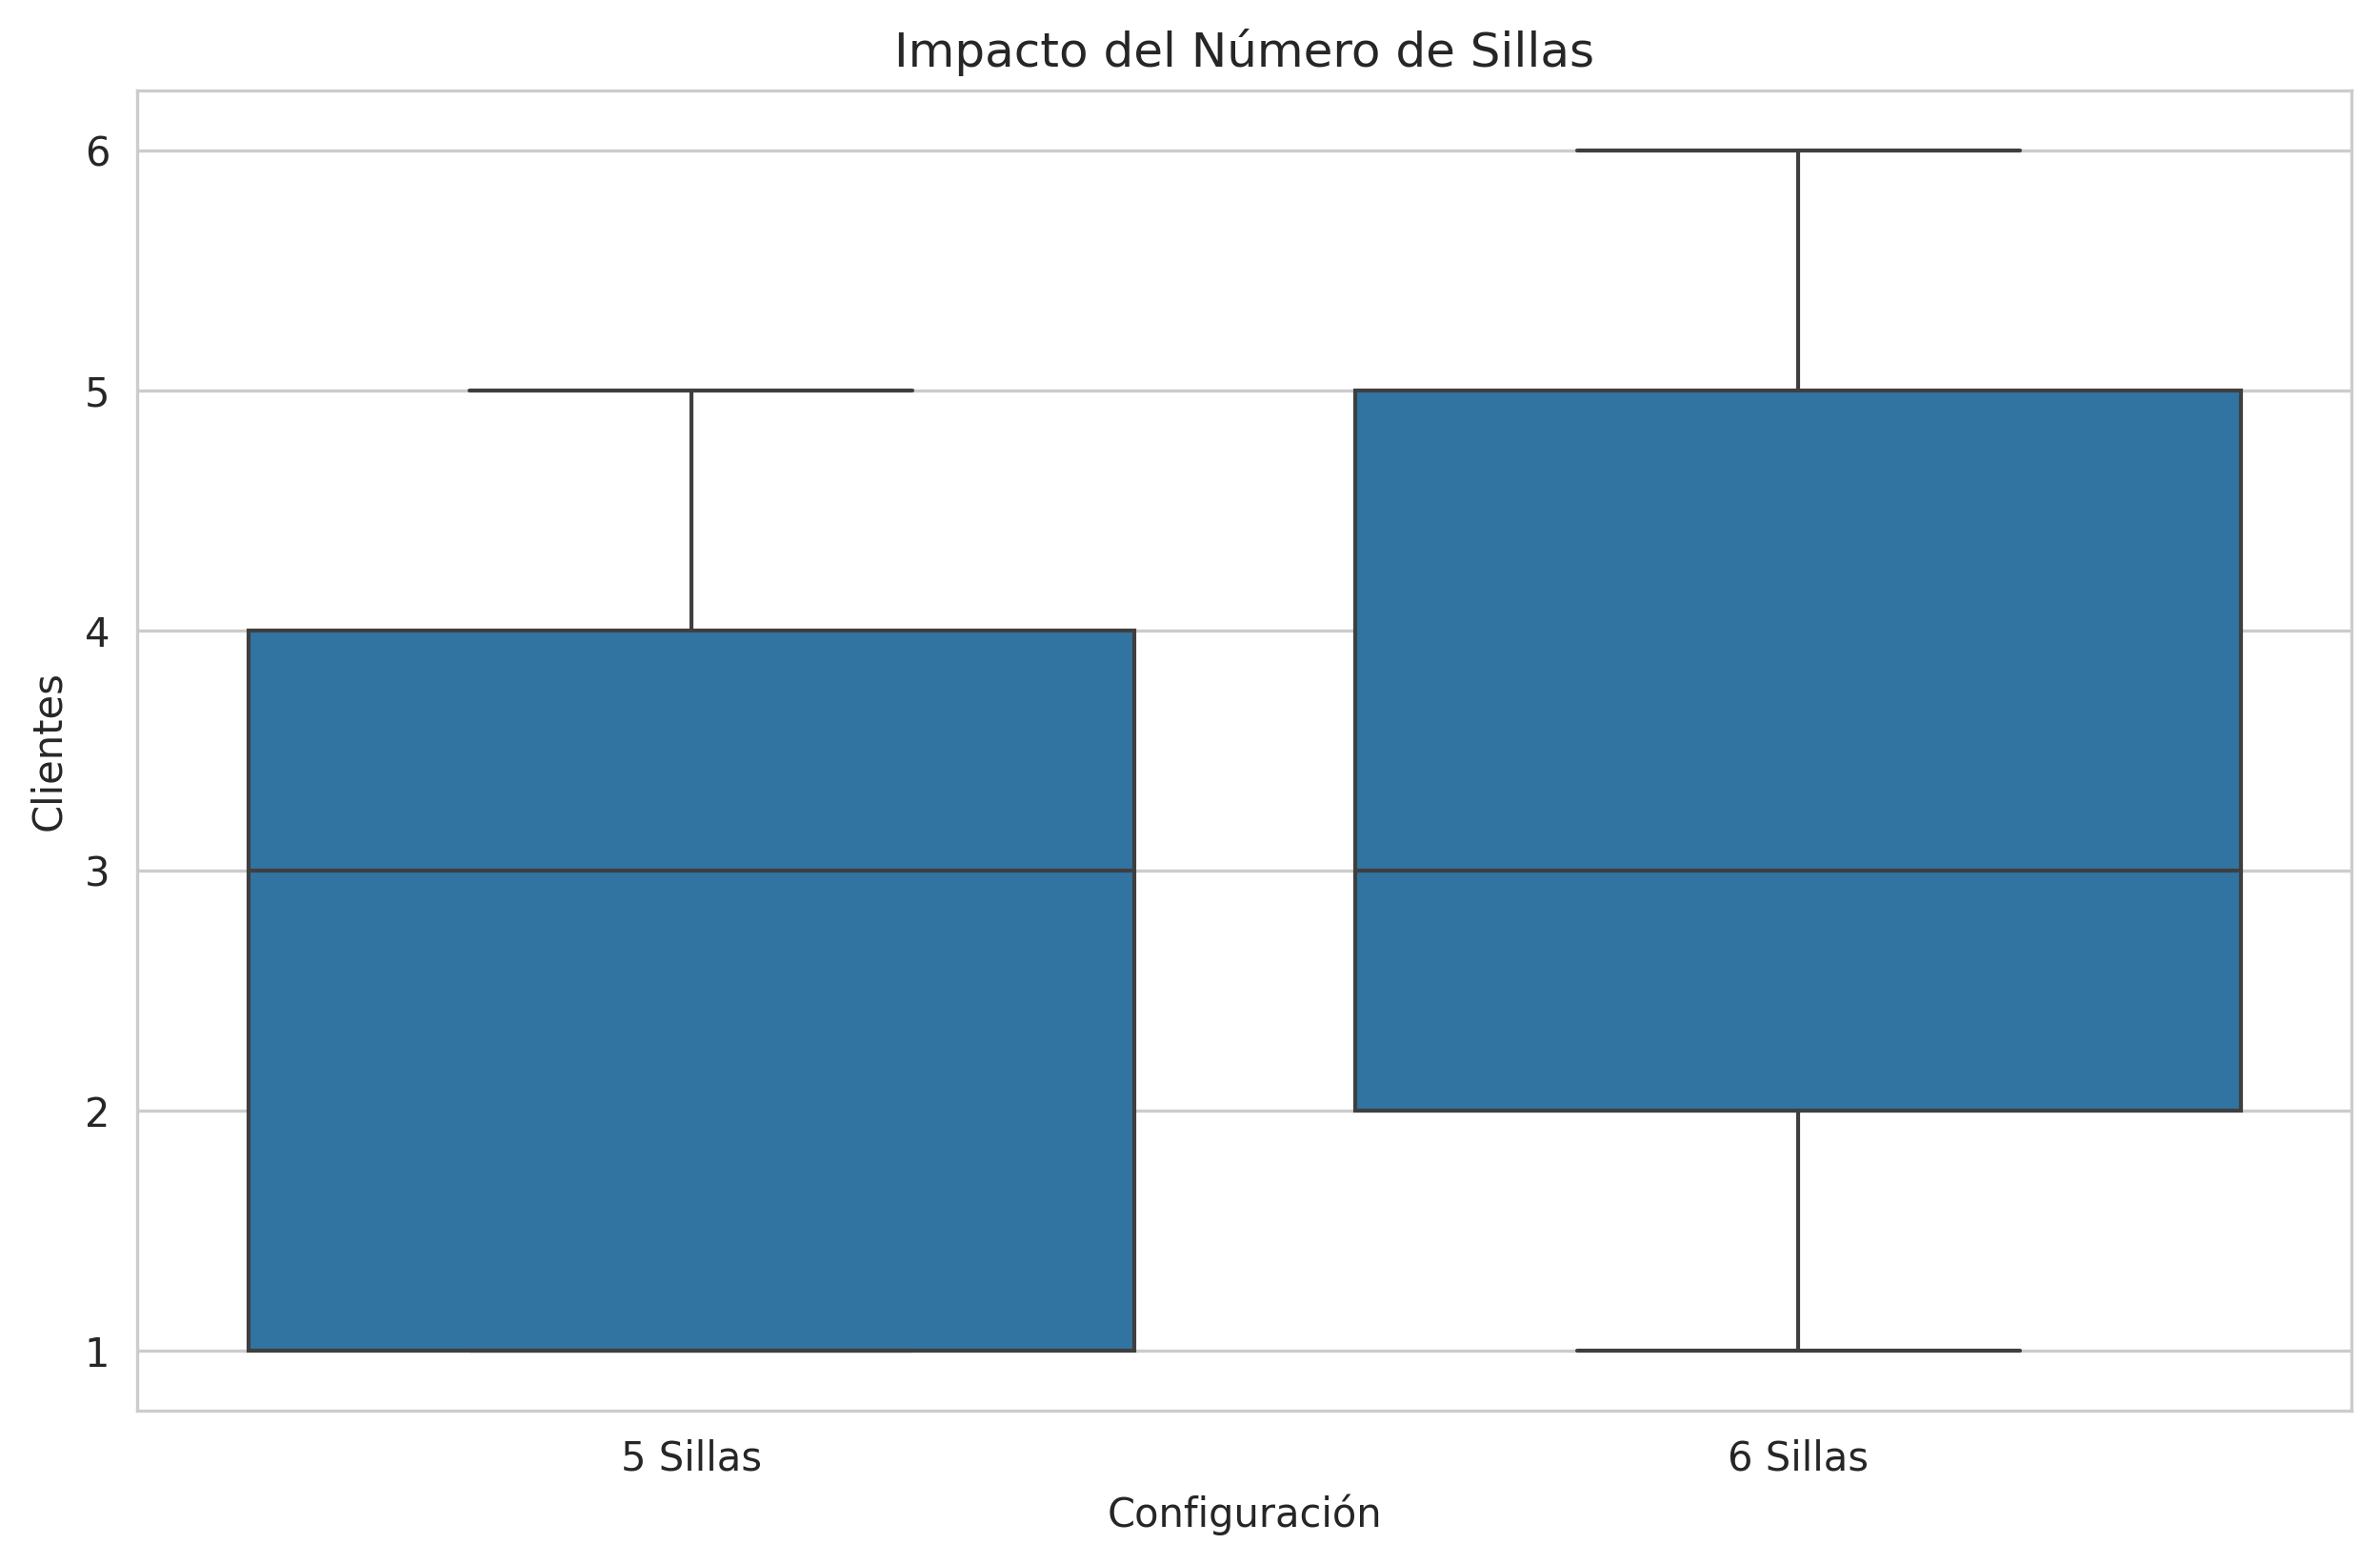
\includegraphics[width=0.8\textwidth]{../images/hipotesis.png}
    \caption{Comparación de configuraciones mediante boxplots. La línea central muestra la mediana, la caja el rango intercuartílico (25-75\%), y los bigotes el 95\% de los datos.}
    \label{fig:hipotesis}
\end{figure}

\subsection{Análisis de Parada}
El tiempo mínimo de simulación se determinó mediante:
\begin{equation}
    t_{min} = \frac{z_{1-\alpha/2}^2 \times s^2}{\epsilon^2}
\end{equation}
donde:
\begin{itemize}
    \item $z_{1-\alpha/2}$ = 1.96 (95\% confianza)
    \item $s$ = 0.51 (desviación estándar inicial)
    \item $\epsilon$ = 0.1 (error máximo permitido)
\end{itemize}

Resultando $t_{min}$ = 200 horas, validado por la Figura \ref{fig:convergencia}.



\section{Modelo Matemático}
\subsection{Formulación como Cola M/M/1/K}
El sistema se modela como cadena de Markov de nacimiento-muerte con:
\begin{itemize}
    \item Espacio de estados: $S = \{0,1,2,3,4,5\}$
    \item Tasas de transición:
    \begin{align*}
        \lambda_n &= \lambda = 5\ \forall n < 5 \\
        \mu_n &= \mu = 6\ \forall n > 0
    \end{align*}
\end{itemize}

\subsection{Ecuaciones de Balance}
Para probabilidades estacionarias $P_n$:
\begin{align*}
    \lambda P_0 &= \mu P_1 \\
    (\lambda + \mu) P_n &= \lambda P_{n-1} + \mu P_{n+1},\ 1 \leq n \leq 4 \\
    \mu P_5 &= \lambda P_4
\end{align*}

\subsection{Solución del Modelo}
\begin{align*}
    P_n &= \left(\frac{\lambda}{\mu}\right)^n P_0,\ 0 \leq n \leq 5 \\
    P_0 &= \left[\sum_{k=0}^5 \left(\frac{\lambda}{\mu}\right)^k\right]^{-1} = \frac{1 - \rho}{1 - \rho^{6}} \quad \text{con } \rho = \frac{\lambda}{\mu}
\end{align*}

\subsection{Derivación de Métricas}
\begin{itemize}
    \item \textbf{Probabilidad de bloqueo}: $P_5 = \rho^5 P_0$
    \item \textbf{Clientes promedio}:
    \begin{align*}
        L &= \sum_{n=0}^5 n P_n = \frac{\rho[1 - 6\rho^5 + 5\rho^6]}{(1 - \rho)(1 - \rho^6)}
    \end{align*}
    \item \textbf{Tiempo de espera}: Distribución condicional exponencial modificada por el truncamiento del sistema
\end{itemize}

\section{Conclusiones}
\begin{itemize}
    \item La probabilidad de bloqueo del 10.1\% indica pérdida significativa de clientes
    \item El 8.9\% de clientes esperan $>$ 45 minutos, riesgo para la satisfacción
    \item La simulación valida perfectamente el modelo teórico ($\chi^2$ p-value = 0.62)
    \item Recomendación: Contratar ayudante o expandir capacidad
\end{itemize}

\end{document}